\chapter{Methodology}

\section{Pipeline}

\subsection{Data Preparation}

As mentioned, the different datasets are distributed in differening formats. A few transformations are done to unify them all as PyTorch datasets.

Due to the preprocessed nature of the ADTOF-YT dataset, the unification is trivial and simply denotes a transformation from a stored TensorFlow dataset to a PyTorch dataset. Otherwise it is kept "as is".

\subsubsection{Audio Files}

The others are however distributed in the Waveform Audio File Format (with the suffix \textit{.wav}) or using the Free Lossless Audio Codec (with the suffix \textit{.flac}). Both of these formats are loaded using the PyTorch library \texttt{Torchaudio} and converted to monophonic format through meaning over each side's waveform. If any datasets contain distinct drum and accompaniement audio (like e.g. ENST-Drums), these are additively mixed together.

After each track is loaded into a waveform, a zero-padding is added to the end of each sequence allowing for even partitioning into 4 second partitions. Then we turn the track into a spectrogram with 2048 fft's, and a window length of 2048. By keeping the hop length equal to the sampling rate divided by 100, the resulting spectrogram's timesteps represent a 10ms window of the original waveform.

After this, a filterbank is computed by generating 12 normalized logarithmically spaced filters, centered at 440Hz, and bounded over the interval [20Hz, 20,000Hz]. Applying this filterbank as a simple matrix multiplication over the spectrogram results in a logarithmically filtered spectrogram with $D_\text{STFT} = 84$ number of frequency bins. Lastly, we turn it into a log-spectrogram by applying a $\log_{10}$ operation to each cell, following an addition of 1 (preventing $\lim_{x \to 0}\log_{10}(x) = -\infty$ situations).

\subsubsection{Annotations}

The annotations are either distributed in specific formats as text files (with the suffix \textit{.txt}), or in MIDI files (with the suffix \textit{.mid} or \textit{.midi}), each one having a different transformation into a sequence of instrument onset probabilities.

The datasets declaring onsets in text files (ENST-Drums and MDB-Drums) follow a similar format, storing onsets on separate lines, each one containing the time in seconds for the onset, and its respective instrument ID, separated by a space or tab respectively. To convert this into the onset probability sequence, we convert the time into a timeframe index by turning the time into milliseconds, dividing by 10 to group into 10ms intervals, and rounding to the nearest integer. After this, we map the instrument ID into its respective class, and set that specific (timeframe, class) cell value to 1.

The data given in MIDI format, the annotations are parsed using the library \texttt{Partitura}, and loads the information into an array of MIDI events called \textit{notes}. These \textit{notes} contain information for each event, importantly time, pitch, and velocity. These events are very thorough, but strict instrument onsets can be isolated by restricting our view to notes with a non-zero velocity. Instruments are denoted by the event's pitch, and a mapping is done from each pitch to a respective class. The time is converted identically to the loading of the text annotations, turning them into timeframe indices. At last, we also here set each specific registered onset (timeframe, class) cell to 1.

In addition to this, we apply a \textit{target widening} step, setting values in timeframes adjacent to an instrument onset with a lower weight, equal to 0.5. This has shown to be benifical in countering sparsity in our labels following multiple works on beat transcription.~\cite{9747048, signals4040042}

\subsubsection{Splitting and Storing}

These spectrogram/onset sequence pairs are stored together in PyTorch's TensorDatasets, separated into each track's respective train/validation/test split, and stored into PyTorch pickle files (with the suffix \textit{.pt}). By doing all this preprocessing in advance, minimal preprocessing has to be done during runtime, increasing the efficiency of training.

\subsection{Preprocessing}

Most of the preprocessing is done during the data preparation step, however there are some remaining. Most importantly, a given model computes the mean and standard deviation of its training dataset, and uses these parameters to standardize its input data before prediction during runtime. 

Data normalization like this has been shown to increase the speed and stability of convergence during training and, in summary, producing models which better generalize to unseen data. Although the specific benefits depend on the normalization technique used, the general consensus is that normalization in itself is beneficial in machine learning, hence their ubiquitous use in state-of-the-art models~\cite{10056354}.

Another preprocessing step motivated by \gls{ADT} specific methods is the use of infrequency weights, which framewise weighs the loss based on the instrument onsets that are present at each frame. These weights are precomputed from the training dataset, and are, for each instrument, computed by what Cartwright and Bello call \textit{"the inverse estimated entropy of their event activity distribution"}~\cite{cartwright2018increasing}. Although they apply this to account for sparsity in data along different tasks, Zehren et al.~\cite{signals4040042} applied it to give more weight to infrequent instruments. 

These weights are computed by calculating the probability of an instrument $i$ appearing $p_i = \frac{n_i}{T}$ as the total number of onsets $n_\text{i}$ divided by the total number of timesteps $T$. With this probability we compute its inverse entropy, giving us our final weights $w_i = (-p_i\log{p_i} - (1 - p_i)\log{1 - p_i})^{-1}$. Note that our probability computation differs from the work of Cartwright and Bello, as we do not divide by the number of instruments~\cite{cartwright2018increasing}. 

\textcolor{red}{Should I mention anything on how the entropy is symmetric over 0.5? Such that a probability over 0.5 would lower our weights again, but how that is not a problem in ADT due to instrument onset inherently being sparse?}

\subsection{Training}

As mentioned, the \gls{ADT} task could be thought of as a sequence labeling task, where we each timeframe could have several instrument onsets present, taking the form of a 0 if an instrument is not present, and a 1 if it is. A natural loss function for this, where each value is handled as a separate independent probability distribution is the binary cross-entropy loss. Due to the numerical instability which can appear by applying a sigmoid activation function to our logits before computing the loss, we instead output our logits directly and utilize PyTorch's \texttt{BCEWithLogitsLoss} loss function, as recommended in their documentation \textcolor{red}{Do I need to cite this?}. It increases the numerical stability by taking advantage of the log-sum-exp trick, increasing numerical precision by avoiding underflow or overflow problems followed by significantly small or large input values.

With the choice by what to use, Adam was considered. This is an optimizer so ubiquitously used within the field of deep learning that when questioned with what optimizer to generally use authors like Sebastian Ruder state that \textit{".., Adam might be the best overall choice}~\cite{ruder2017overviewgradientdescentoptimization}. However contrary to this, the Adam optimizer has been shown to contain some issues, like its coupling of the weight decay term inside its gradient-based updates. Due to this, the choice instead fell on AdamW, a modified Adam implementation decoupling weight decay in whole from the gradient-based updates, and displaying a better ability to generalize.~\cite{kingma2017adammethodstochasticoptimization, bock2018improvementconvergenceproofadamoptimizer, loshchilov2019decoupledweightdecayregularization}

It was observed during training that the magnitude of the loss values could vary greatly and often displayed a tendancy to explode. To counteract this observation, we clip the gradients with a maximum norm set to 2. This addition significantly lowered the observed chance of exploding gradients occuring. 

Another addition which is frequenct in other \gls{ADT} works is the use of a learning rate scheduler. A learning rate scheduler keeps track of recent validation loss values, and if the minimum loss achieved plateaus (meaning it stop decreasing) for a certain number of epochs, the learning rate gets reducing by a given factor. In this thesis we reduce the learning rate by a factor of 5 if we observe 5 epochs of plateauing, with no improvement to our minimal validation loss~\cite{chang2024yourmt3multiinstrumentmusictranscription, signals4040042}. We also keep track of the general count of epochs since validation loss last improvement and perform an early stop if we ever observe 15 epochs without improvement (this is hightened to 25 epochs for the smallest dataset, ENST+MDB).

\subsection{Evaluation}

\subsubsection{Postprocessing}

As mentioned, the model outputs a sequence of activation values, a 2 dimensional matrix with values on the interval $(0, 1)$ interpreted as the model's confidence in an instrument onset being present per frame. This can be utilized directly when computing our loss during training, however it is a difficult format to work with when talking about general performance, due to it rather representing a continuous confidence rather than discrete predictions. To suit this purpose, additional postprocessing is performed on the output.

First, we apply the aforementioned peak picking algorithm to isolate peaks in the model's onset confidence, intuitively being frames where the model is most confident in an instrument onset happening ~\cite{Bck2012EvaluatingTO, vogl2018multiinstrumentdrumtranscription}. Afterwards, we count a predicted onset if the given peak has a value larger or equal to 0.5. From this, it is trivial to compare predicted onsets with actual onsets, by greedily iterating our output sequence from the beginning, counting a prediction as a true positive if it happens within a 5 frame (50 ms) interval of a true onset, false positive if it happens outside such an interval, or false negative if a true onset happens with no prediction within said interval.

\begin{figure}[H]
    \centering
    %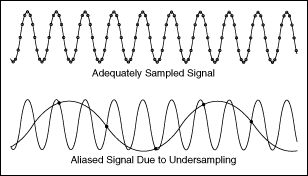
\includegraphics[scale=2.0]{figures/signalaliasing.png}
    \textcolor{red}{Could be useful showing transformation from output, to peak picked, to correct vs incorrect prediction.}
    %\caption{Example of aliasing in an undersampled signal.}
    %\label{AliasingFigure}
\end{figure}

These \gls{TP}, \gls{FP}, \gls{FN} predictions are then added together and used to compute the previously mentioned micro F1-score. For additional analysis, we also compute and store instrumentwise F1-scores.

\textcolor{red}{Mention the loss function used, and why we use this (BCEWithLogitsLoss).}

\textcolor{red}{Mention the computation of infrequency weights, i.e. how they are computed, why they are computed, the intuition into how they will help us...}

\textcolor{red}{Also write how we evaluate our models. E.g count up TP, FP, FN, and compute micro F1-score after finishing the whole split.}

\section{Experiments}

\textcolor{red}{Here we mention the setups for each of the experiments.}

\textcolor{red}{Mention that we use RayTune to train, with PyTorch models. Mention that we only used RayTune's FIFOScheduler, and how for random search / grid search we used their built in parameter space functionality.}

\textcolor{red}{Mention that every single experiment was trained for at most 100 epochs, with a early stopping if validation loss didn't decrease within 10 epochs.
Mention the learning rate scheduler, where we reduce the learning rate by a factor of 5 if the model hasn't improved in the last 3 epochs.}

\textcolor{red}{Mention that we perform early stopping on the validation loss (and why, like the smooth nature, overfitting prevention, etc.), where as we store the best performing model based on the validation F1-score (due to this representing overall prediction performance).}

\textcolor{red}{Mention that every experiment is model selected using hold-out validation, and best model is chosen based on micro F1-score.}